\chapter{Introduction}

The greatest challenge in remote sensing is being able to produce a classified image without the need for human input. One advantage of this is for hazard mapping. The Gorkha earthquake struck Nepal in April 2015, killing ~9000 people and damaging a 550 by 200km region of Nepal. Following the earthquake, there was an extremely large humanitarian effort to map all the areas that had been affected by landslides so that aid could be distributed effectively (\cite{kargel16}). If classified imagery could have been downloaded directly from the provider at the point of use, aid could have been sent to the most at-risk areas a lot sooner.
\par
Currently, image classification methods are split into two types, object-based classification and pixel-based classification (\cite{chen18}), this is shown in Figure \ref{fig.pix_vs_obj}. 
\begin{figure}[htpb]

\centering
\begin{subfigure}{0.35\textwidth}
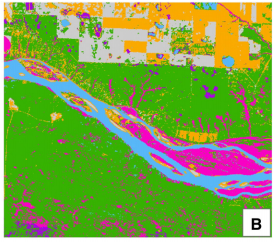
\includegraphics[width=\textwidth]{\dir/figs/pixel.png}
\caption{Pixel-wise decision tree}
\label{fig.pixel-based}
\end{subfigure}%
\qquad
\begin{subfigure}{0.35\textwidth}
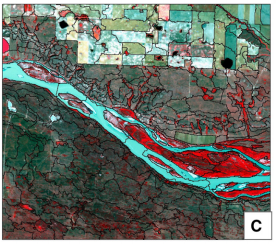
\includegraphics[width=\textwidth]{\dir/figs/mrs15_object.png}
\caption{Object-based using multi-resolution segmentation}
\label{fig.object-based}
\end{subfigure}
\caption{Comparison of image classification techniques, adapted from \cite{duro12}.}
\label{fig.pix_vs_obj}
\end{figure}
In object-based methods, the pixels are grouped according to similar spectra and textural characteristics and then segmented (Figure \ref{fig.object-based}) (\cite{martha11}). The accuracy of this method is dependent on the thresholds that are manually adjusted for different cases, leading to uncertainties. In pixel-based classification (Figure \ref{fig.pixel-based}), the class is mapped pixel by pixel reducing the segmentation and need for manually defined thresholds (\cite{hussain13}). Some of these classification techniques look at the spectral characteristics of each pixel and assign it to a class. More advanced techniques combine information from neighbouring pixels to enhance the performance of the classifier. These two pixel-based techniques are not viable on a large scale because they rely on the separability of different classes based on the spectrum of a single-pixel or neighbouring pixels. In large scale satellite imagery, high spectral resolution is not always available so it becomes difficult to identify pixels based on their spectrum. Additionally, due to the large scale variability over entire datasets with high spatial extent, there are issues due to increased inter-class variability (\cite{maggiori17b}).
\par
Due to the recent explosion in very high resolution imagery (VHR), there is now a need for an automatic classification method to reduce the processing time that is required for the current models. There are only a few semi-automated systems and no fully automated systems in existence (\cite{baltsavias04,mayer08,mnih13}). Deep learning, therefore, is gaining traction as a method for pixel-based classification as it exploits feature representations based exclusively from data rather than handcrafted features that are designed based on domain-specific knowledge (\cite{xiao17,maggiori17a}). 
\paragraph{}
\subsection*{Neural Networks}
Neural Networks (NN) are a method of deep learning that have been used to classify images. At their most basic level, NNs transform data from feature space to class space. They belong to the same class of techniques as automated pattern recognition (\cite{Ritter89}), regression and spatial classifications. Parametric supervised classifiers such as Maximum Likelihood Classifiers (MLC) assume the data has a normal distribution and are limited for use with multi-modal input datasets (\cite{Liu11}). Neural networks main advantage over these traditional parametric statistical approaches is that they are distribution free, no assumptions are used to model the underlying distribution of the data in feature space (\cite{Patricia97}). All Neural networks are made up of neurons with learnable weights and biases. Random Forests (RF) (\cite{belgiu16,Breiman01}) and Support Vector Machine (SVM) (\cite{cortes95,vapnik82}) learning are examples of neural networks that are widely used in the field of remote sensing. A new and emerging neural network from the field of computer vision are Convolutional Neural Networks, which make assumptions about the underlying data that will be discussed at the end of this section. 
% \subsubsection{Random Forests}
% RFs are an ensemble classifier that produces multiple decision trees using a randomly selected subset of training samples (\cite{Breiman01}). They have successfully been used to select and rank variables with the greatest ability to distinguish between target classes. This is an important feature for remote sensing where the high dimensionality of data makes the selection of the most relevant variables, time-consuming (\cite{belgiu16}). RF is an ensemble based classifier that uses classification based regression trees (Figure \ref{fig.random_forest}) based on individual or multiple classifiers and trained using bagging (\cite{belgiu16}). Each classifier in the ensemble is trained on a random subset of the training sample set.

% \begin{figure}[htpb]
%     \centering
%     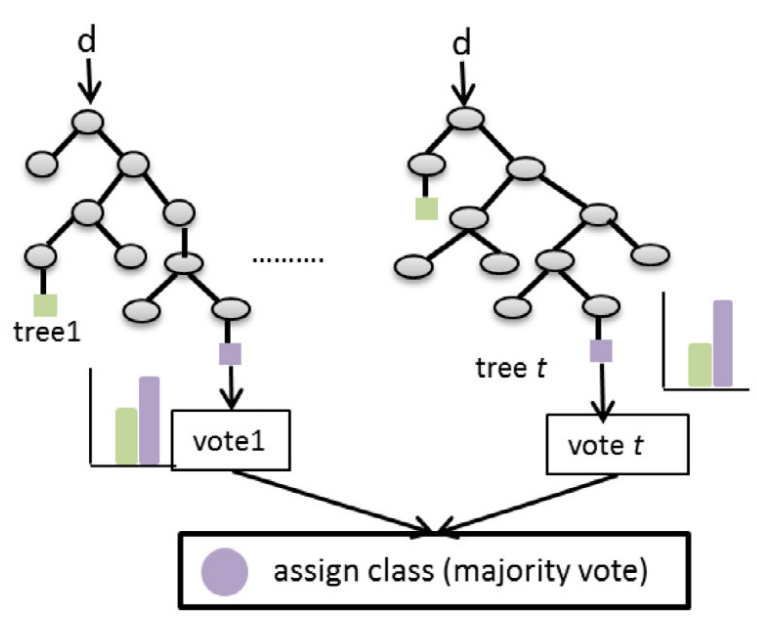
\includegraphics[width=0.5\textwidth]{\dir/figs/random_forest.PNG}
%     \caption[An example of classifying using Random Forests]{An example of how bagging works to classify pixels while using the Random Forest Classifier. Each tree is classified based on which class received the most votes during training. Taken from \citet{belgiu16}.}
%     \label{fig.random_forest}
% \end{figure}
% \subsubsection{Support Vector Machine}
% SVMs are a form of non-parametric statistical learning technique that makes no assumptions about the underlying data distribution (\cite{vapnik82}). The method is presented with a set of labelled data instances and the SVM attempts to find a hyperplane (Figure \ref{fig.svm_hyperplane}) that separates the dataset into discrete instances while minimising the number of misclassifications. SVMs are appealing in the field of remote sensing due to their ability to successfully handle small training sets, producing higher classification accuracy than traditional methods (\cite{cortes95}).
% \begin{figure}[htpb]
%     \centering
%     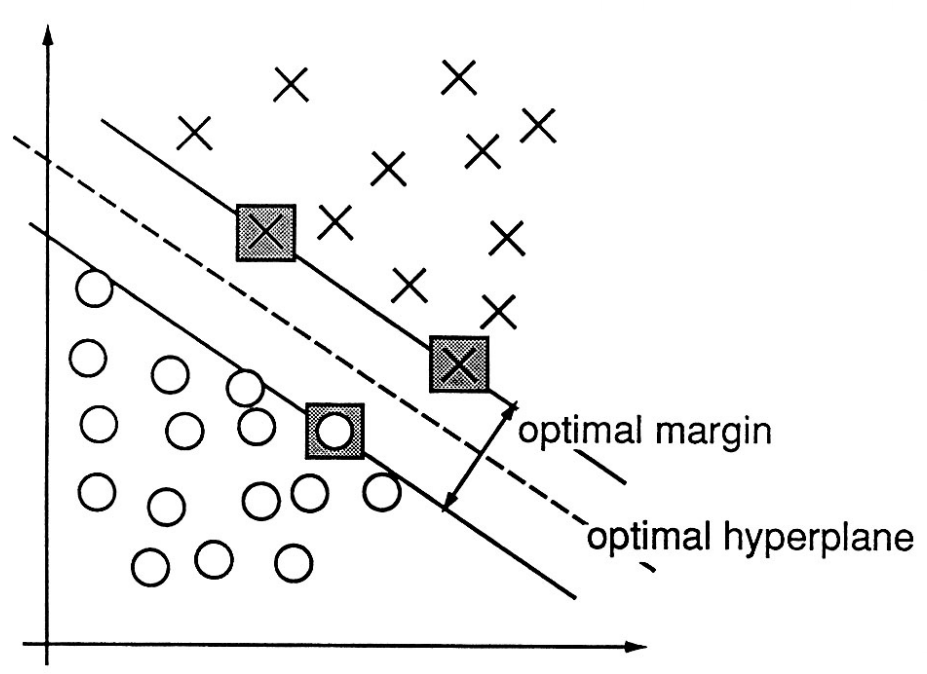
\includegraphics[width=0.5\textwidth]{\dir/figs/hyperplane_svm.png}
%     \caption[An example of finding the hyperplane for Support Vector Machine Learning]{An example of a finding the hyperplane in a 2-dimensional space. The method is the same for multi-dimensional space and works to define the largest separation between the number of classes present (\cite{cortes95}).}
%     \label{fig.svm_hyperplane}
% \end{figure}
\subsubsection{Convolutional Neural Networks}
CNNs are a trainable, multi-stage architecture specifically designed to work well for inputs with multiple channels, i.e. images. They are made up of multiple neurons with learnable weights and biases, just like RFs and SVMs.  (\cite{Karpathy1}). CNNs are a distinct class of neural networks because they explicitly assume that the inputs are images allowing for certain properties to be encoded. Regular neural networks, using RFs and SVMs, do not scale well to images with multiple channels of information. For remote sensing classification problems, the imagery will have at least three channels of information, if not more. For a regular neural network, a 256x256 pix image with three channels equates to 196,000 weights to calculate per neuron, requiring a lot of parameters and can lead to overfitting. CNNs take advantage of the 3D volume of neurons so that each of the neurons has a height, width and depth component where the depth corresponds to the number of channels in the input image. Each stage of the network has inputs and outputs that are \textit{feature maps}, each \textit{feature map} represents a particular feature extracted from the input (\cite{lecun10}).
\par
CNNs have been inspired by the biological process as the network patterns resemble that of the animal visual cortex. They require relatively little pre-processing when compared to other classification algorithms, the network learns how to classify the image wherein other classification algorithms the classifier needs to train the algorithm manually. Compared to other neural networks, CNNs have fewer connections and parameters and so are easier to train with their theoretical best performance only being slightly less (\cite{krizhevsky17}). 

\begin{figure}[htpb]
    \centering
    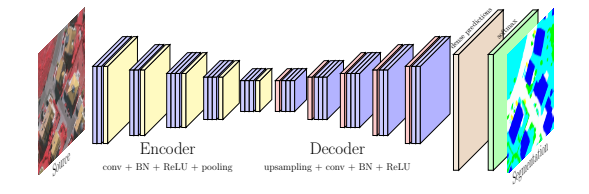
\includegraphics[width=0.9\textwidth]{\dir/figs/segnet.png}
    \caption{SegNet architecture for semantic labelling, taken from \cite{audebert18}}
    \label{fig.segnet}
\end{figure}
The paper by \cite{long15} outlines how a fully convolutional neural network (FCN), that has been trained end-to-end, pixels-to-pixels, can exceed existing procedures (\cite{shelhamer17}). Figure \ref{fig.segnet} shows an example of the SegNet architecture to classify a scene using encoder-decoder to produce an output with the same resolution as the original scene (\cite{audebert18}). CNNs were designed for image classification tasks, i.e. assigning a single class label to an entire image (\cite{volpi17}). The first example of a successful CNN for image classification was a result of the ILSVRC challenge in 2012, where CNNs outperformed start-of-the-art classification systems (\cite{marmanis16,volpi17,krizhevsky17}). 
\paragraph{}
The objective of this project is to produce a set of procedures that can be replicated by other remote sensing researchers to train and develop a CNN for their specific problem. The work presented here is a workflow for other researchers to build upon in their search for a semi-automated classification system using the most up to date deep learning techniques.
 


